\section{Alpine} \label{sec:results_alpine}

We refer to an alpine climate, here, as one that experiences below zero temperatures during certain periods of the year. These extreme temperatures ensure that only plant species able to survive in sub-zero temperatures will persist in the long term. It is possible, however, for annuals to sprout during periods when the temperature increases.\\

In this section resources are configured, clusters generated and plausible vegetation distributions computed and analysed in the same manner as done previously in section \ref{sec:results_trop_rainforest}. These tests differ in their input resource configurations and plant species, however, in order to better model an alpine climate. \\
Verbier, a Swiss alpine city at a latitude of 43\textdegree north, is the location on which input climate data is based. See table \ref{tab:results_alpine_input_resources} for details concerning this input data. To more accurately represent the drastic change in temperature that occurs in alpine climates, the lapse rate is changed from its default and set to a ten degree drop in temperature for every thousand metres altitude gain. To model a drier loamy soil as for the previous tests, the soil infiltration rate is set to ten millimetres per hour (see figure \ref{tab:soil_types}). Rocky cliff faces are modelled with the soil infiltration rate set to zero for slope angles surpassing forty-five degrees. Figure \ref{fig:results_alpine_water_networks} shows the monthly water networks that form as a result of the configured rainfall and soil properties. \\
\textit{Spruce}, \textit{Maple}, \textit{Moss Campion}, \textit{Daisy} and \textit{Beech} are the five species which are used for these tests. Refer to appendix \ref{AppendixF} for the resource requirements associated with each.\\

\definecolor{green}{rgb}{0,1,0}
\begin{table}[htb!]
  \centering
	    \begin{tabular}{|p{3cm}|p{.7cm}|p{.7cm}|p{.7cm}|p{.7cm}|p{.7cm}|p{.7cm}|p{.7cm}|p{.7cm}|p{.7cm}|p{.7cm}|p{.7cm}|p{.7cm}|}
		\hline	
  	    \textbf{Resource} & \textbf{Jan} & \textbf{Feb} & \textbf{Mar} & \textbf{Apr} & \textbf{May} & \textbf{Jun} & \textbf{Jul} & \textbf{Aug} & \textbf{Sep} & \textbf{Oct} & \textbf{Nov} & \textbf{Dec} \\
  	    \hline	
		Rainfall (mm) & \cellcolor{green}57 & \cellcolor{green}49 & \cellcolor{green}41 & \cellcolor{green}27 & \cellcolor{green}42 & \cellcolor{green}51 & \cellcolor{green}42 & \cellcolor{green}42 & \cellcolor{green}46 & \cellcolor{green}48 & \cellcolor{green}52 & \cellcolor{green}63  \\
		\hline
		Rainfall Intensity (mm/h) & \cellcolor{green}16 & \cellcolor{green}12 & \cellcolor{green}11 & \cellcolor{green}7 & \cellcolor{green}11 & \cellcolor{green}14 & \cellcolor{green}11 & \cellcolor{green}11 & \cellcolor{green}12 & \cellcolor{green}13 & \cellcolor{green}14 & \cellcolor{green}17  \\
		\hline
		Soil Moisture (mm) & 36 & 41 & 37 & 27 & 38 & 36 & 38 & 38 & 38 & 37 & 37 & 37  \\
		\hline
		Weighted soil moisture (mm)	& 36 & 38	& 38 & 32 & 34 & 35 & 38 & 38 & 38 & 38 & 37 & 37 \\
		\hline
		Temperature (\textdegree) & 5 & 10 & 15 & 20 & 25 & \cellcolor{green}30 & 25 & 20 & 15 & 10 & 5 & \cellcolor{green}0  \\
		\hline
		\end{tabular}
		\caption{\textit{Alpine: Monthly rainfall, rainfall intensity, soil moisture, weighted soil moisture and temperature at zero metres. Green cells represent values explicitly input for this test scenario, all others are procedurally calculated. The soil moisture is valid for terrain vertices with a slope less than forty-five degrees and therefore for which the soil infiltration rate is 10 mm per hour. All other vertices have a soil moisture of zero (modelled rock cliff faces).}}
	  \label{tab:results_alpine_input_resources}
\end{table}

\begin{figure}[htb!]
\center
	\includegraphics[width=\textwidth]{results_alpine_water_networks.png}
	\caption{\textit{Alpine: Water networks that form on the terrain in every month. From left to right, top to bottom.}}
	\label{fig:results_alpine_water_networks}
\end{figure}

Figure \ref{fig:results_alpine_terrain_clusters} illustrates the clustered terrain. Corresponding cluster properties are summarized in figure \ref{fig:results_alpine_cluster_hum_temp_illum} and table \ref{tab:results_alpine_cluster_slope_covarea}. 

\begin{figure}[htb!]
\center
	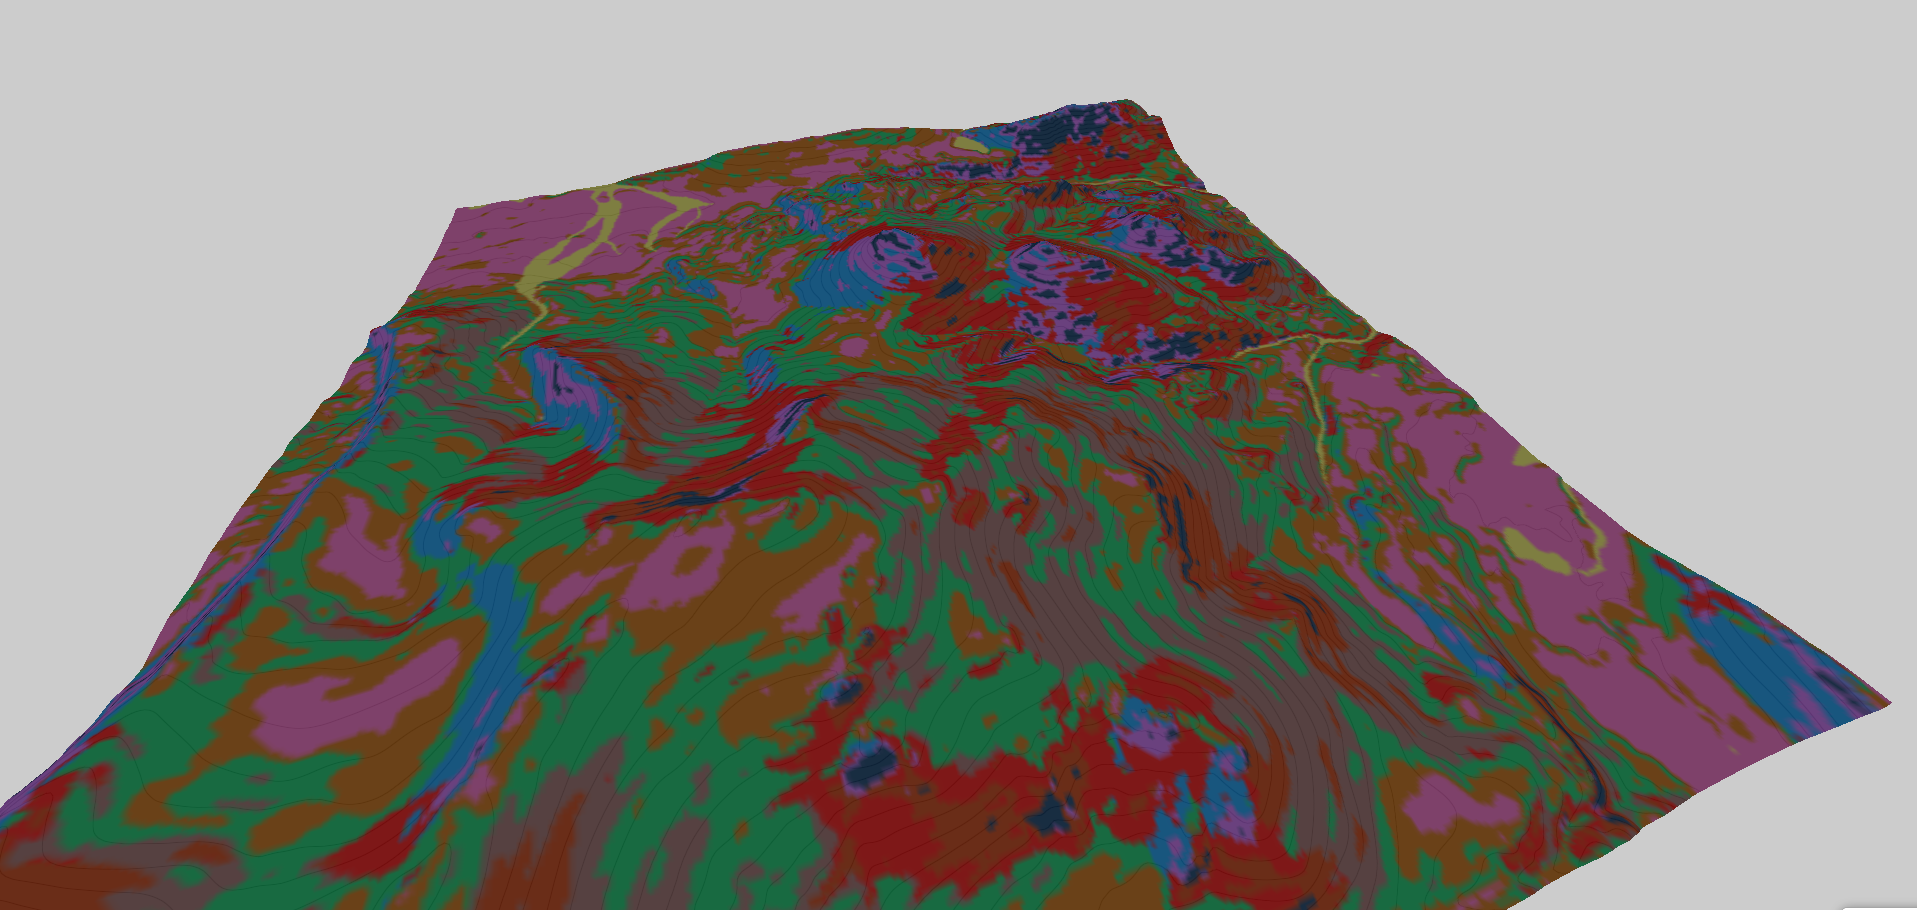
\includegraphics[width=\textwidth]{results_alpine_clusters_on_terrain.png}
	\caption{\textit{Alpine: Resulting terrain clusters.}}
	\label{fig:results_alpine_terrain_clusters}
\end{figure}

\begin{figure}[htb!]
\center
	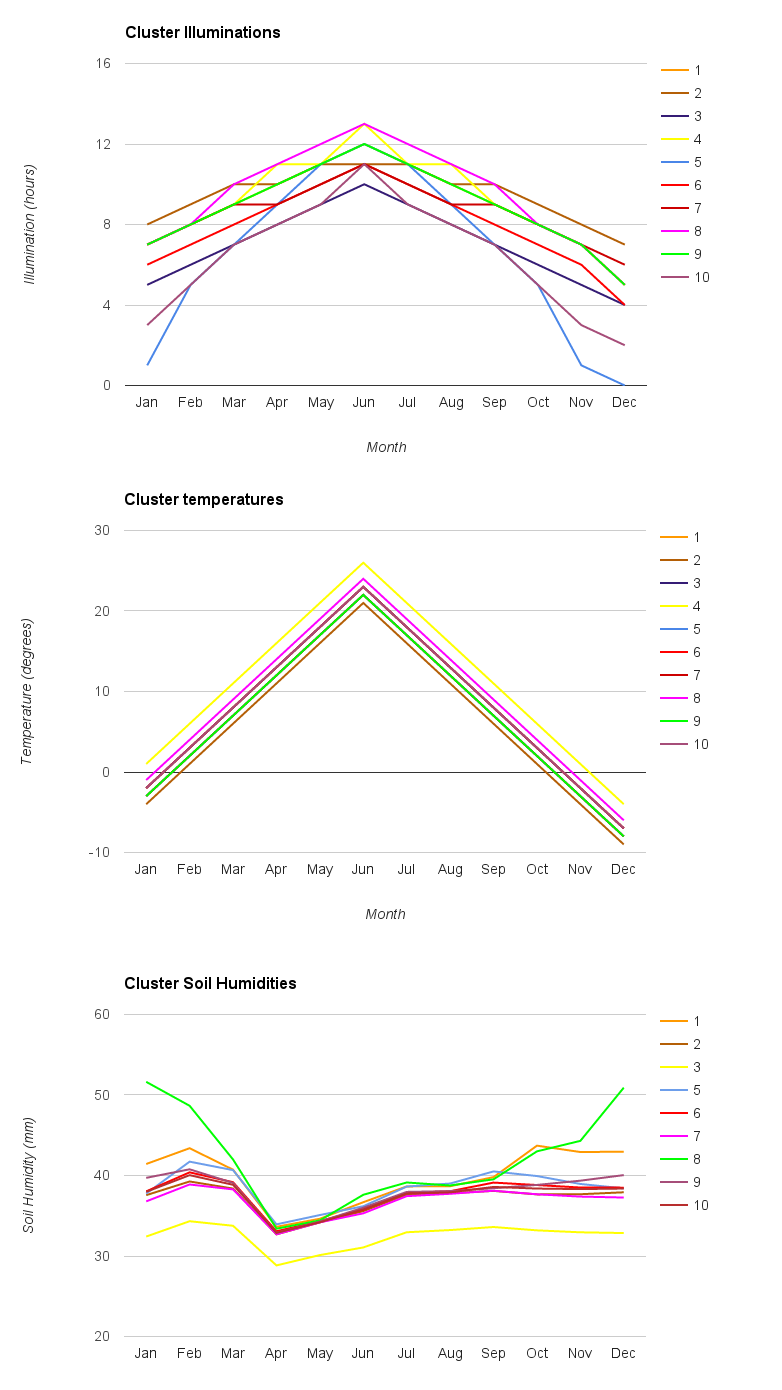
\includegraphics[height=\textheight-60pt,keepaspectratio]{results_alpine_clusters_hum_illum_temp.png}
	\caption{ \textit{Alpine: Mean monthly sun exposure (top), temperatures (middle) and soil moistures (bottom) for each terrain cluster. Note that soil humidity data is removed for cluster 4 because the values are too high.}}
	\label{fig:results_alpine_cluster_hum_temp_illum}
\end{figure}

\begin{table}[htb!]
  \centering
	    \begin{tabular}{|p{5cm}|p{5cm}|p{5cm}|}
		\hline	
  	    Cluster & \textbf{Slope (degrees)} & \textbf{Coverage area (\% of terrain)} \\
  	    \hline	
		Cluster 1 & 10.2 & 18 \\
		\hline
		Cluster 2 & 21.1 & 13.5 \\
		\hline
		Cluster 3 & 35.8 & 3.7 \\
		\hline
		Cluster 4 & 5.3 & 2 \\
		\hline
		Cluster 5 & 19.9 & 4.2 \\
		\hline
		Cluster 6 & 22.3 & 10.4 \\
		\hline
		Cluster 7 & 28.2 & 9.3 \\
		\hline
		Cluster 8 & 5 & 15 \\
		\hline
		Cluster 9 & 15.7 & 19.4 \\
		\hline
		Cluster 10 & 28.7 & 4.2 \\
		\hline
		\end{tabular}
		\caption{\textit{Alpine: Slope and coverage area associated with each cluster}}
	  \label{tab:results_alpine_cluster_slope_covarea}
\end{table}

The results of the specie suitability filtering step is summarized in figure \ref{tab:results_alpine_species_suitability}. As stated previously, this step filters out species from being inserted into given clusters because the temperature, slope or soil moisture is ill-suited. From this, it is possible to conclude that no plants are able to grow, and therefore no ecosystem simulator needs to be run, for cluster 4. This is caused by excess moisture as this cluster represents areas on the terrain covered in water.\\ 
This data also shows that Daisies are only suited to grow in cluster 8. In all other clusters, the temperature drops below its minimum. It is important to note that, even though Daisies are a season plant, in order for them to be considered for growth at any time in the year, the temperature must be above the species absolute minimum all year round. If the temperature drops below this absolute minimum, it is considered too cold for even the seeds to survive through the winter. Cluster 8 is suited for this seasoned plant as the minimum annual temperature is -6 degrees, one degree higher than the species absolute minimum. At this temperature, it is too cold for the given species to grow but is sufficiently high for the seeds to survive in order to sprout in the warmer summer months.\\

\definecolor{color_red}{rgb}{1.0,0.0,0.0}
\definecolor{color_green}{rgb}{0.0,1.0,0.0}
\definecolor{color_orange}{rgb}{1.0,0.65,0.0}

\begin{table}[htb!]
  \centering
	    \begin{tabular}{|p{2cm}|p{2.5cm}|p{2.5cm}|p{2.5cm}|p{2.5cm}|p{2.5cm}|}
		\hline	
		&  \textbf{Spruce} & \textbf{Maple} & \textbf{Moss Campion} & \textbf{Daisy} & \textbf{Beech}\\
		\hline	
		Cluster 1 & 
		Y & 
		Y & 
		Y & 
		\cellcolor{color_red}N (T$^{-}$) & 
		Y \\
		\hline	
		Cluster 2 & 
		Y & 
		Y & 
		Y & 
		\cellcolor{color_red}N (T$^{-}$) & 
		Y \\
		\hline	
		Cluster 3 & 
		\cellcolor{color_red}N (S$^{+}$) & 
		Y & 
		Y & 
		\cellcolor{color_red}N (T$^{-}$) & 
		Y \\
		\hline	
		Cluster 4 & 
		\cellcolor{color_red}N (SH$^{+}$) & 
		\cellcolor{color_red}N (SH$^{+}$) & 
		\cellcolor{color_red}N (SH$^{+}$) & 
		\cellcolor{color_red}N (SH$^{+}$) & 
		\cellcolor{color_red}N (SH$^{+}$) \\
		\hline	
		Cluster 5 & 
		Y & 
		Y & 
		Y & 
		\cellcolor{color_red}N (T$^{-}$) & 
		Y \\
		\hline	
		Cluster 6 & 
		Y & 
		Y & 
		Y & 
		\cellcolor{color_red}N (T$^{-}$) & 
		Y \\
		\hline	
		Cluster 7 & 
		Y & 
		Y & 
		Y & 
		\cellcolor{color_red}N (T$^{-}$) & 
		Y \\
		\hline	
		Cluster 8 & 
		Y & 
		Y & 
		Y & 
		Y &
		Y \\
		\hline	
		Cluster 9 & 
		Y & 
		Y & 
		Y & 
		\cellcolor{color_red}N (T$^{-}$) & 
		Y \\
		\hline	
		Cluster 10 &
		Y & 
		Y & 
		Y & 
		\cellcolor{color_red}N (T$^{-}$) & 
		Y \\
		\hline	
		\end{tabular}
		\caption{\textit{Alpine: Summary of the species suitability filter pass on each cluster. This step filters out ill-suited species from being inserted into a given cluster is the slope, soil humidity or temperature is ill-suited. If a species is not suited, the cell is highlighted red and the reason is stated in brackets where \textit{S} is the slope, \textit{T} is the temperature and \textit{SH} is the soil humidity, $^{+}$ signifies too much and $^{-}$ too little of the given resource.}}
	  \label{tab:results_alpine_species_suitability}
\end{table}

To visualise each species suitability to the given clusters in terms of temperature, soil moisture and sun exposure, graphs similar to those plotted in the tropical tests (section \ref{sec:results_trop_rainforest}) are plotted (see figures \ref{fig:results_alpine_spruce_suitability}, \ref{fig:results_alpine_maple_suitability}, \ref{fig:results_alpine_moss_campion_suitability}, \ref{fig:results_alpine_daisy_suitability} and \ref{fig:results_alpine_beech_suitability}). Table \ref{tab:results_alpine_species_slope_suitability} summarizes the species suitability in terms of slope. From this data, it is possible to conclude that: Available illumination drops beneath the minimum permitted for all species in clusters \textit{3, 5, 6} and \textit{10}; Illumination in clusters \textit{1, 8} and \textit{9} also falls beneath the lower limit for \textit{Moss Campion, Daisy} and \textit{Beech}; Illumination in cluster 7 also prevents \textit{Daisy} and \textit{Beech} from surviving. In summary, only clusters one, two, seven, eight and nine are able to support plant development. Together, they make up seventy-five percent of the terrain.\\

\begin{figure}[htb!]
\center
	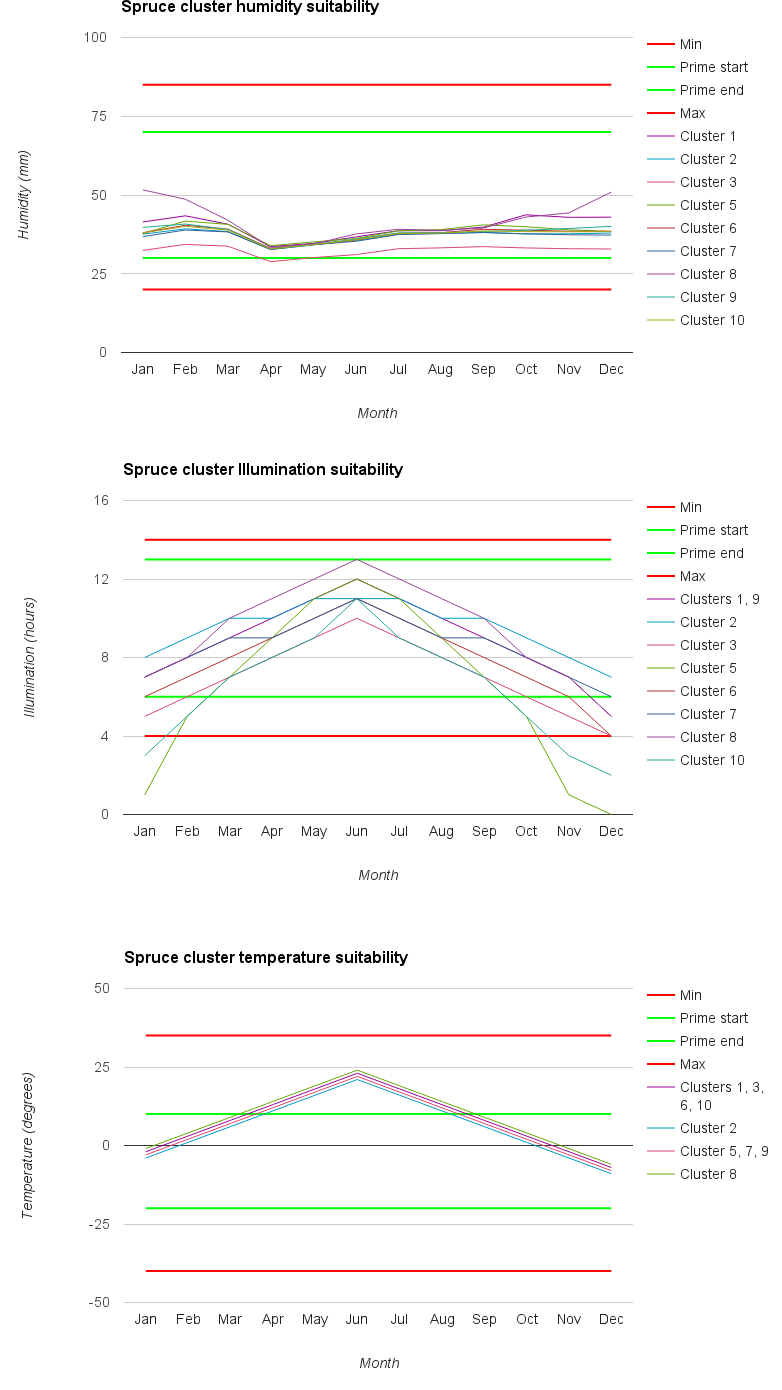
\includegraphics[height=\textheight-60pt,keepaspectratio]{spruce_suitability.png}
	\caption{ \textit{Alpine: Spruce suitability to clusters 1, 2, 3, 5, 6, 7, 8, 9 and 10 in terms of temperature (top-left), illumination (top-right) and soil humidity (bottom). The thick green lines and red lines delimit the species prime range and absolute limits respectively.}}
	\label{fig:results_alpine_spruce_suitability}
\end{figure}

\begin{figure}[htb!]
\center
	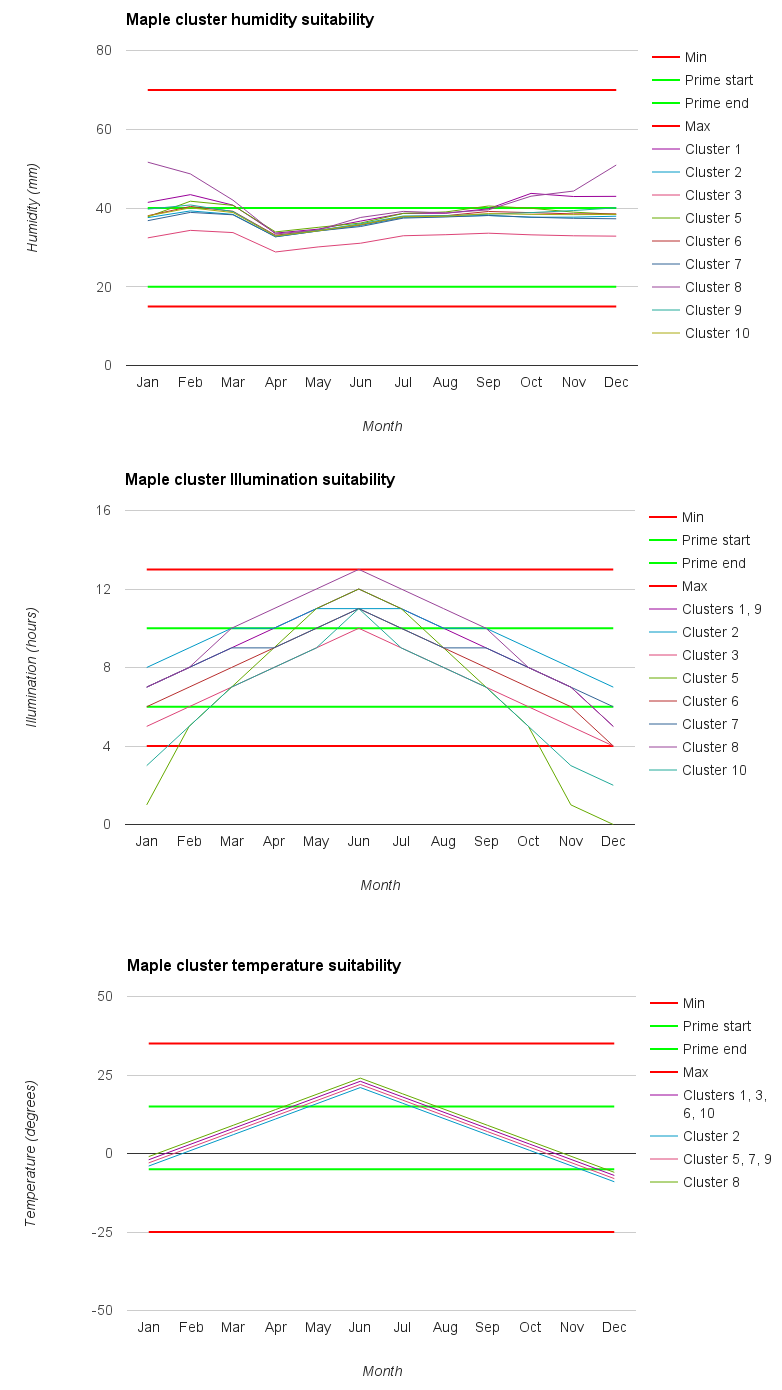
\includegraphics[height=\textheight-60pt,keepaspectratio]{maple_suitability.png}
	\caption{ \textit{Alpine: Maple suitability to clusters 1, 2, 3, 5, 6, 7, 8, 9 and 10 in terms of temperature (top-left), illumination (top-right) and soil humidity (bottom). The thick green lines and red lines delimit the species prime range and absolute limits respectively.}}
	\label{fig:results_alpine_maple_suitability}
\end{figure}

\begin{figure}[htb!]
\center
	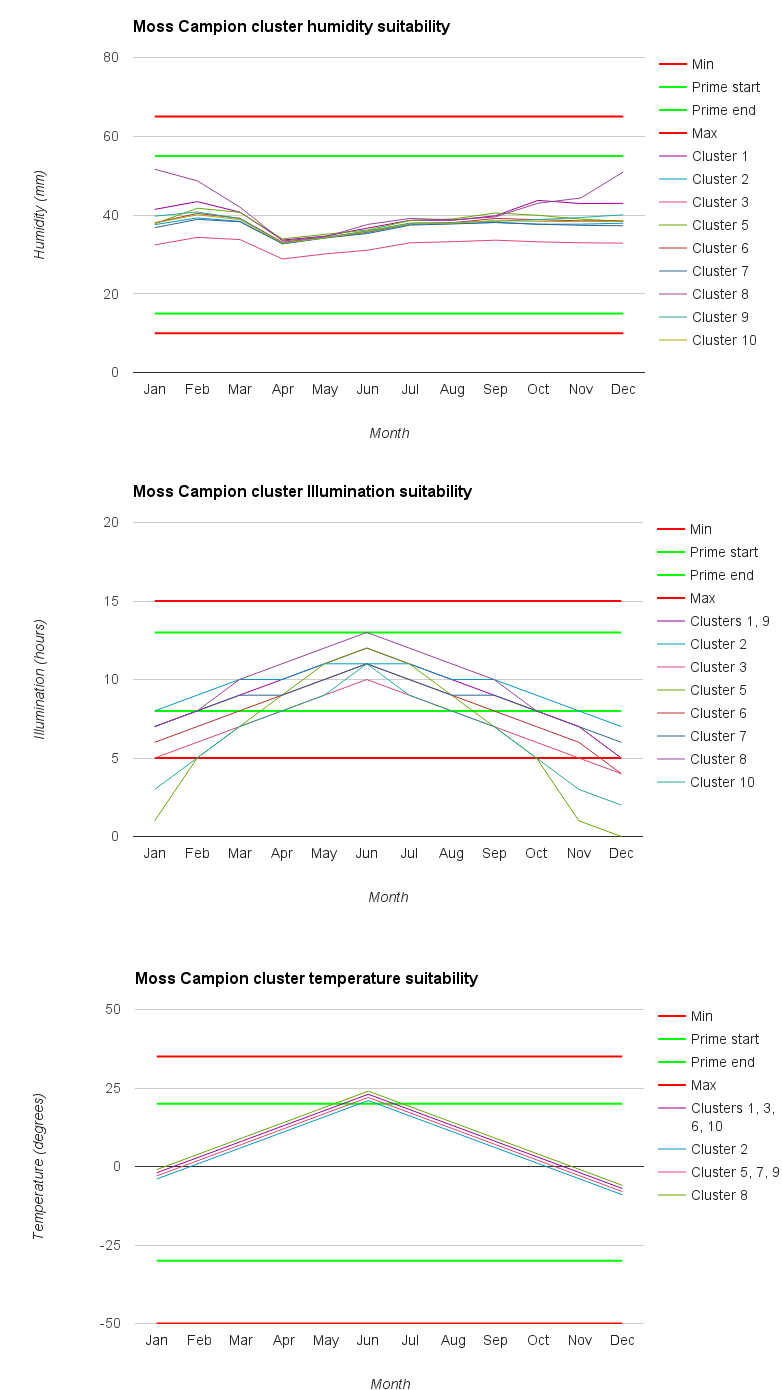
\includegraphics[height=\textheight-60pt,keepaspectratio]{moss_campion_suitability.png}
	\caption{ \textit{Alpine: Moss Campion suitability to clusters 1, 2, 3, 5, 6, 7, 8, 9 and 10 in terms of temperature (top-left), illumination (top-right) and soil humidity (bottom). The thick green lines and red lines delimit the species prime range and absolute limits respectively.}}
	\label{fig:results_alpine_moss_campion_suitability}
\end{figure}

\begin{figure}[htb!]
\center
	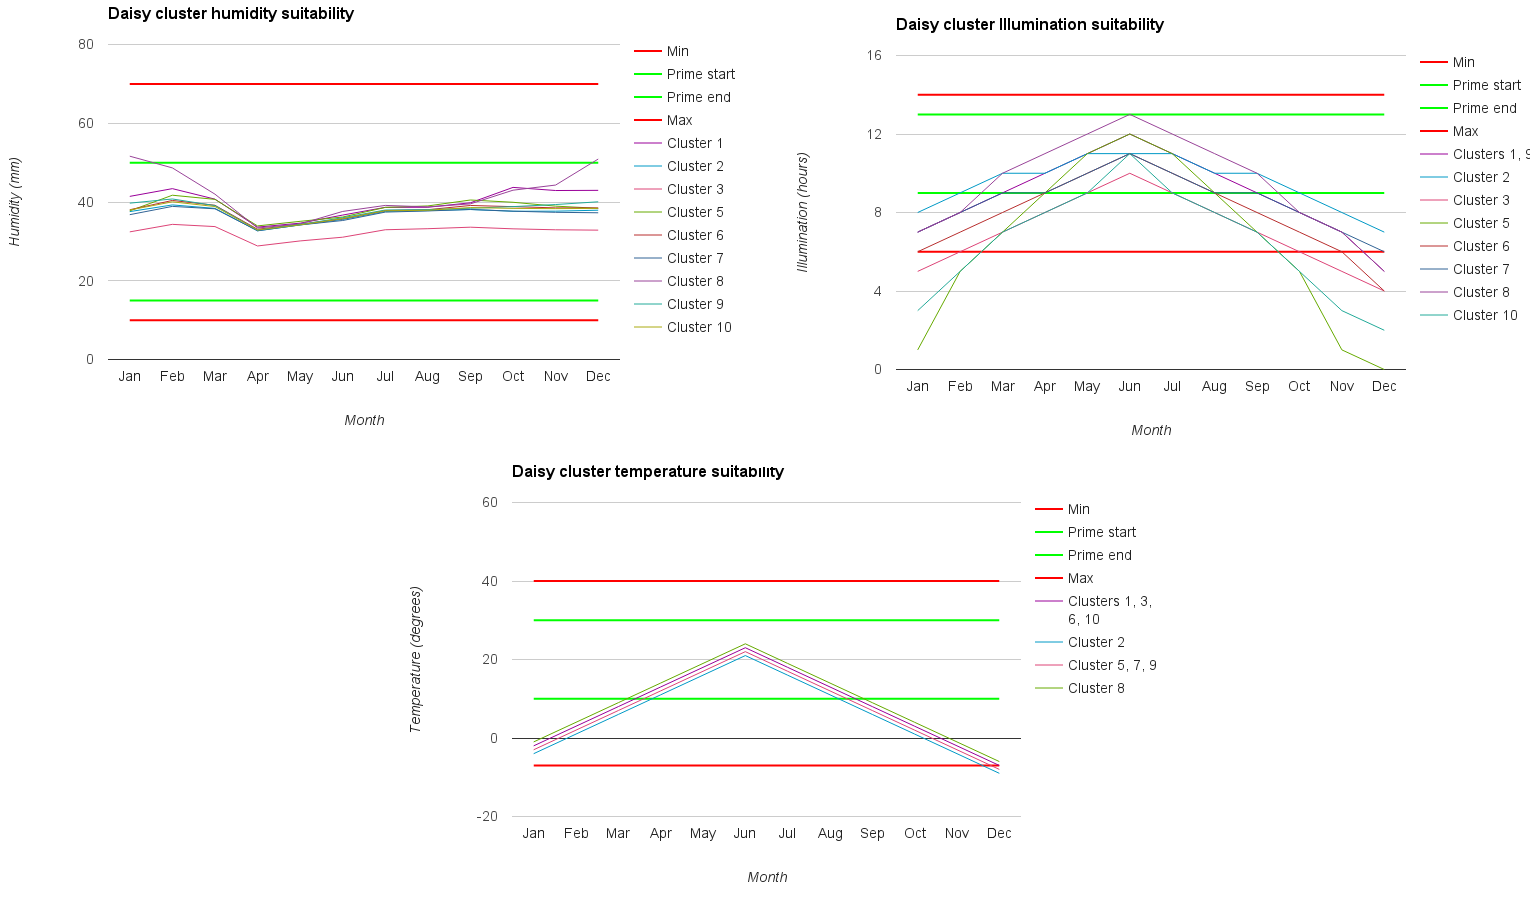
\includegraphics[height=\textheight-60pt,keepaspectratio]{daisy_suitability.png}
	\caption{ \textit{Alpine: Daisy suitability to clusters 1, 2, 3, 5, 6, 7, 8, 9 and 10 in terms of temperature (top-left), illumination (top-right) and soil humidity (bottom). The thick green lines and red lines delimit the species prime range and absolute limits respectively.}}
	\label{fig:results_alpine_daisy_suitability}
\end{figure}

\begin{figure}[htb!]
\center
	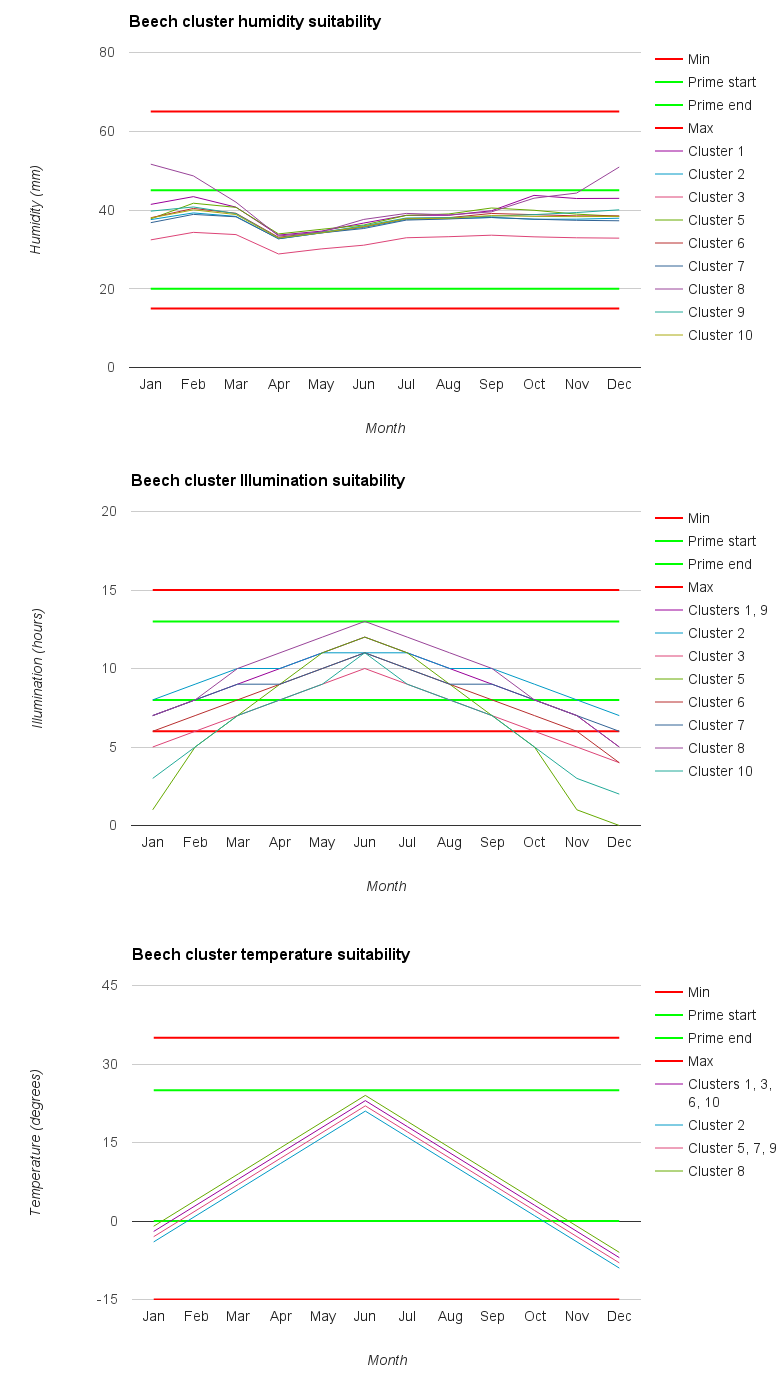
\includegraphics[height=\textheight-60pt,keepaspectratio]{beech_suitability.png}
	\caption{ \textit{Alpine: Beech suitability to clusters 1, 2, 3, 5, 6, 7, 8, 9 and 10 in terms of temperature (top-left), illumination (top-right) and soil humidity (bottom). The thick green lines and red lines delimit the species prime range and absolute limits respectively.}}
	\label{fig:results_alpine_beech_suitability}
\end{figure}

\begin{table}[htb!]
  \centering
	    \begin{tabular}{|p{2cm}|p{2.5cm}|p{2.5cm}|p{2.5cm}|p{2.5cm}|p{2.5cm}|}
		\hline	
  	     & \textbf{Spruce} & \textbf{Maple} & \textbf{Moss Campion} & \textbf{Daisy} & \textbf{Beech}\\
  	    \hline	
		\textbf{Start of decline} & 
		25 & 
		15 & 
		66 & 
		50 & 
		10 \\
		\hline
		\textbf{Max} & 
		50 & 
		30 & 
		90 & 
		75 & 
		40 \\
		\hline
		\textbf{Cluster 1} & 
		\cellcolor{color_green}10.2 &
		\cellcolor{color_green}10.2 &
		\cellcolor{color_green}10.2 &
		\cellcolor{color_green}10.2 &
		\cellcolor{color_orange}10.2 \\
		\hline
		\textbf{Cluster 2} & 
		\cellcolor{color_orange}21.1 &
		\cellcolor{color_orange}21.1 &
		\cellcolor{color_green}21.1 &
		\cellcolor{color_green}21.1 &
		\cellcolor{color_orange}21.1 \\
		\hline
		\textbf{Cluster 3} & 
		\cellcolor{color_orange}35.8 & 
		\cellcolor{color_red}35.8 & 
		\cellcolor{color_green}35.8 & 
		\cellcolor{color_green}35.8 & 
		\cellcolor{color_orange}35.8\\
		\hline
		\textbf{Cluster 5} & 
		\cellcolor{color_green}19.9 & 
		\cellcolor{color_orange}19.9 & 
		\cellcolor{color_green}19.9 & 
		\cellcolor{color_green}19.9 & 
		\cellcolor{color_orange}19.9\\
		\hline
		\textbf{Cluster 6} & 
		\cellcolor{color_green}22.3 & 
		\cellcolor{color_orange}22.3 & 
		\cellcolor{color_green}22.3 & 
		\cellcolor{color_green}22.3 & 
		\cellcolor{color_orange}22.3\\
		\hline
		\textbf{Cluster 7} & 
		\cellcolor{color_orange}28.2 & 
		\cellcolor{color_orange}28.2 & 
		\cellcolor{color_green}28.2 & 
		\cellcolor{color_green}28.2 & 
		\cellcolor{color_orange}28.2\\
		\hline
		\textbf{Cluster 8} & 
		\cellcolor{color_green}5 & 
		\cellcolor{color_green}5 & 
		\cellcolor{color_green}5 & 
		\cellcolor{color_green}5 & 
		\cellcolor{color_green}5\\
		\hline
		\textbf{Cluster 9} & 
		\cellcolor{color_green}15.7 & 
		\cellcolor{color_orange}15.7 & 
		\cellcolor{color_green}15.7 & 
		\cellcolor{color_green}15.7 & 
		\cellcolor{color_orange}15.7\\
		\hline
		\textbf{Cluster 10} & 
		\cellcolor{color_orange}28.7 & 
		\cellcolor{color_orange}28.7 & 
		\cellcolor{color_green}28.7 & 
		\cellcolor{color_green}28.7 & 
		\cellcolor{color_orange}28.7\\
		\hline
		\end{tabular}
		\caption{\textit{Alpine: Species suitability to clusters 1 to 10 (excluding 4) in terms of slope, where: Green means the species is completely suited, orange means the species is negatively impacted by the slope, and red that the species is completely ill-suited. All values are in \textit{degrees}.}}
	  \label{tab:results_alpine_species_slope_suitability}
\end{table}

\begin{table}[htb!]
  \centering
	    \begin{tabular}{|p{2cm}|p{2cm}|p{1.5cm}|p{1.5cm}|p{1.5cm}|p{1.5cm}|p{1.5cm}|}
		\hline	
		\textbf{Specie} & \textbf{Property} & \textbf{Cluster 1} & \textbf{Cluster 2} & \textbf{Cluster 7} & \textbf{Cluster 8} & \textbf{Cluster 9} \\
		\hline
		% Spruce 1
		\multirow{4}{*}{\textbf{Spruce}} & 
						\multicolumn{1}{l|}{Count} & 
						\multicolumn{1}{l|}{3112} & 
						\multicolumn{1}{l|}{3242} &
						\multicolumn{1}{l|}{3916} & 
						\multicolumn{1}{l|}{3272} & 
						\multicolumn{1}{l|}{3395} \\\cline{2-7} &
						\multicolumn{1}{l|}{Min height (cm)} & 
						\multicolumn{1}{l|}{1} & 
						\multicolumn{1}{l|}{1} &
						\multicolumn{1}{l|}{1} &
						\multicolumn{1}{l|}{1} & 
						\multicolumn{1}{l|}{1} \\\cline{2-7} &
						\multicolumn{1}{l|}{Max height (cm)} & 
						\multicolumn{1}{l|}{137} & 
						\multicolumn{1}{l|}{166} &
						\multicolumn{1}{l|}{130} &
						\multicolumn{1}{l|}{131} & 
						\multicolumn{1}{l|}{143} \\\cline{2-7} &
						\multicolumn{1}{l|}{Avg height (cm)} & 
						\multicolumn{1}{l|}{70} & 
						\multicolumn{1}{l|}{87} &
						\multicolumn{1}{l|}{67} &
						\multicolumn{1}{l|}{66} & 
						\multicolumn{1}{l|}{73} \\\cline{2-6}
		\hline       
		% Maple 2
		\multirow{4}{*}{\textbf{Maple}} & 
						\multicolumn{1}{l|}{Count} & 
						\multicolumn{1}{l|}{556} & 
						\multicolumn{1}{l|}{850} &
						\multicolumn{1}{l|}{0} &
						\multicolumn{1}{l|}{24} & 
						\multicolumn{1}{l|}{528} \\\cline{2-7} &
						\multicolumn{1}{l|}{Min height (cm)} & 
						\multicolumn{1}{l|}{3} & 
						\multicolumn{1}{l|}{1} &
						\multicolumn{1}{l|}{-} & 
						\multicolumn{1}{l|}{2} &
						\multicolumn{1}{l|}{3} \\\cline{2-7} &
						\multicolumn{1}{l|}{Max height (cm)} & 
						\multicolumn{1}{l|}{481} & 
						\multicolumn{1}{l|}{146} &
						\multicolumn{1}{l|}{-} & 
						\multicolumn{1}{l|}{3} &
						\multicolumn{1}{l|}{520} \\\cline{2-7} &
						\multicolumn{1}{l|}{Avg height (cm)} & 
						\multicolumn{1}{l|}{248} & 
						\multicolumn{1}{l|}{72} &
						\multicolumn{1}{l|}{-} & 
						\multicolumn{1}{l|}{2} &
						\multicolumn{1}{l|}{289} \\\cline{2-7}
		\hline      
		%Moss Campion 4 
		\multirow{4}{*}{\textbf{MC}} & 
						\multicolumn{1}{l|}{Count} & 
						\multicolumn{1}{l|}{0} & 
						\multicolumn{1}{l|}{3239} &
						\multicolumn{1}{l|}{2432} &
						\multicolumn{1}{l|}{0} & 
						\multicolumn{1}{l|}{0} \\\cline{2-7} &
						\multicolumn{1}{l|}{Min height (cm)} & 
						\multicolumn{1}{l|}{-} &
						\multicolumn{1}{l|}{1} & 
						\multicolumn{1}{l|}{1} &
						\multicolumn{1}{l|}{-} & 
						\multicolumn{1}{l|}{-} \\\cline{2-7} &
						\multicolumn{1}{l|}{Max height (cm)} & 
						\multicolumn{1}{l|}{-} & 
						\multicolumn{1}{l|}{16} &
						\multicolumn{1}{l|}{14} &
						\multicolumn{1}{l|}{-} & 
						\multicolumn{1}{l|}{-} \\\cline{2-7} &
						\multicolumn{1}{l|}{Avg height (cm)} & 
						\multicolumn{1}{l|}{-} & 
						\multicolumn{1}{l|}{9} &
						\multicolumn{1}{l|}{7} &
						\multicolumn{1}{l|}{-} & 
						\multicolumn{1}{l|}{-} \\\cline{2-7}
		\hline      
		% Daisy 5
		\multirow{4}{*}{\textbf{Daisy}} & 
						\multicolumn{1}{l|}{Count} & 
						\multicolumn{1}{l|}{0} & 
						\multicolumn{1}{l|}{0} &
						\multicolumn{1}{l|}{0} &
						\multicolumn{1}{l|}{2} & 
						\multicolumn{1}{l|}{0} \\\cline{2-7} &
						\multicolumn{1}{l|}{Min height (cm)} & 
						\multicolumn{1}{l|}{-} &
						\multicolumn{1}{l|}{-} & 
						\multicolumn{1}{l|}{-} &
						\multicolumn{1}{l|}{8} & 
						\multicolumn{1}{l|}{-} \\\cline{2-7} &
						\multicolumn{1}{l|}{Max height (cm)} & 
						\multicolumn{1}{l|}{-} &
						\multicolumn{1}{l|}{-} & 
						\multicolumn{1}{l|}{-} &
						\multicolumn{1}{l|}{8} & 
						\multicolumn{1}{l|}{-} \\\cline{2-7} &
						\multicolumn{1}{l|}{Avg height (cm)} & 
						\multicolumn{1}{l|}{-} &
						\multicolumn{1}{l|}{-} & 
						\multicolumn{1}{l|}{-} &
						\multicolumn{1}{l|}{8} & 
						\multicolumn{1}{l|}{-} \\\cline{2-7}
		\hline     
		% Beech 3
		\multirow{4}{*}{\textbf{Beech}} & 
						\multicolumn{1}{l|}{Count} & 
						\multicolumn{1}{l|}{0} & 
						\multicolumn{1}{l|}{914} &
						\multicolumn{1}{l|}{0} &
						\multicolumn{1}{l|}{0} & 
						\multicolumn{1}{l|}{0} \\\cline{2-7} &
						\multicolumn{1}{l|}{Min height (cm)} & 
						\multicolumn{1}{l|}{-} &
						\multicolumn{1}{l|}{1} & 
						\multicolumn{1}{l|}{-} &
						\multicolumn{1}{l|}{-} & 
						\multicolumn{1}{l|}{-} \\\cline{2-7} &
						\multicolumn{1}{l|}{Max height (cm)} & 
						\multicolumn{1}{l|}{-} &
						\multicolumn{1}{l|}{173} & 
						\multicolumn{1}{l|}{-} &
						\multicolumn{1}{l|}{-} & 
						\multicolumn{1}{l|}{-} \\\cline{2-7} &
						\multicolumn{1}{l|}{Avg height (cm)} & 
						\multicolumn{1}{l|}{-} &
						\multicolumn{1}{l|}{85} & 
						\multicolumn{1}{l|}{-} &
						\multicolumn{1}{l|}{-} & 
						\multicolumn{1}{l|}{-} \\\cline{2-7}
		\hline                                                       
		\end{tabular}
	\caption{\textit{Alpine: Vegetation content of the hundred by hundred metre simulation window for each cluster. MC is Moss Campion.}}
	\label{tab:results_alpine_species_cluster_properties}	
\end{table}

Table \ref{tab:results_alpine_species_cluster_properties} gives an overview of the suitability of each specie and cluster pair by providing the plant instance count along with the minimum, maximum and average plant size. We discuss each cluster below.\\

\paragraph{Cluster one}

A low monthly illumination of five hours in December prevents \textit{Moss Campion} and \textit{Beech} plants from surviving in this cluster.\\
With just over five hundred and fifty instances, \textit{Maple} plants are able to survive in this cluster. With an average height of just over a fifth of the maximum, resources are not optimal. Many of these plants are still growing, however, as at one hundred year (simulation time), only 60\% of the growth period has been completed. With this factored in, these plants are at just over a third of their maximum size. The factors preventing optimal growth of \textit{Maple} plants in this cluster are too much rainfall in the winter months and too much sun exposure and heat exposure in the summer months.\\
The growth potential of \textit{Spruce} in this cluster is very similar to that of \textit{Maple}. Although humidity and sun exposure are better suited to the \textit{Spruce}, they are more sensitive to and ill-affected by the high summer temperatures.

\paragraph{Cluster two}

This is the cluster with the most biodiversity, with four out of the five available species able to survive.\\
As with cluster one, \textit{Spruce} struggles to grow during the summer months due to high temperatures. However, as these highs are a bit less severe in this cluster, growth does improve. With an average height of just under 90 centimetres, they reach just over a third of there maximum size.\\
Similarly, \textit{sun exposure} and \textit{temperature} are more suitable in this cluster for \textit{Maple} plants. Soil humidity is also optimal all year round. With an average height of 146 centimetres, approximately 20\% of the species maximum, however, \textit{Maple} plants are severely affected by the slope of this cluster (21 \textdegree).\\
With over three thousand instances and an average size of over half of the species maximum, Moss Campion plants are the most suited to this cluster. December is the only month in which Moss Campion growth is ill-affected, caused by low sunlight exposure.\\
\textit{Beech} plants are also able to survive in this cluster, but, because of low winter temperatures and limited sunlight exposure in December, these plants only reach 20\% of their maximum size.

\paragraph{Cluster seven}

A combination of high summer temperatures and a slope very close to the species upper-limit prevents \textit{Maple} plants from developing in this cluster.\\
Low sunlight exposure in December also prevents this cluster from being suitable for the growth of \textit{Beech} plants.\\
\textit{Spruce} is able to grow but, with an average size of only a fourth of the species optimum, are unable to reach their maximum growth potential. High summer temperatures and slope are the limiting factor here.\\
The environment is also suited to \textit{Moss Campion} growth. Low sun exposure during winter months and high peak summer temperatures limits growth to just under 50\% of the maximum, however.\\

\paragraph{Cluster eight}

Although \textit{Daisies} are able to grow in this cluster as it is the only one for which the temperature stays above this species lower limit, because the temperature is below its prime range for seven months of the year, growth is limited. In addition, illumination is also below this species optimal range for five months. Because of this, the average daisy height is only a fifth of its maximum size, clearly showing that this habitat is from from optimal.\\
A very small number of Maple plants (twenty-four) are present in this cluster and with an average height of two centimetres, very far from its maximum of twelve metres, it is evident this species struggles. A combination of too much water in the winter months along with too much heat and sun in the summer months proves to be a complete bottleneck for \textit{Maple} growth in this cluster. Given how much this species is struggling, it is clear that the habitat is inadequate. So much so that its presence in this cluster is questionable altogether. As an extension to this work, a final filtering could be performed on the output of the ecosystem simulator to remove species which don't reach a minimum ratio of their maximum.\\
The species that strives best is \textit{Spruce}. However, with an average height of just over a quarter of the species maximum, available resources are far from ideal. Although humidity and illumination is optimal all year round, high summer temperatures have a negative impact on growth.\\

\paragraph{Cluster nine}

Low sunlight exposure in the month of December prevents \textit{Beech} and \textit{Moss Campion} growth in this cluster.\\
\textit{Spruce} plants are able to grow but are affected by high summer temperatures and low sun exposure in December. The same factors negatively impact the growth of \textit{Maple} within this cluster.\\